% Options for packages loaded elsewhere
\PassOptionsToPackage{unicode}{hyperref}
\PassOptionsToPackage{hyphens}{url}
\PassOptionsToPackage{dvipsnames,svgnames,x11names}{xcolor}
%
\documentclass[
  letterpaper,
  DIV=11,
  numbers=noendperiod]{scrartcl}

\usepackage{amsmath,amssymb}
\usepackage{lmodern}
\usepackage{iftex}
\ifPDFTeX
  \usepackage[T1]{fontenc}
  \usepackage[utf8]{inputenc}
  \usepackage{textcomp} % provide euro and other symbols
\else % if luatex or xetex
  \usepackage{unicode-math}
  \defaultfontfeatures{Scale=MatchLowercase}
  \defaultfontfeatures[\rmfamily]{Ligatures=TeX,Scale=1}
\fi
% Use upquote if available, for straight quotes in verbatim environments
\IfFileExists{upquote.sty}{\usepackage{upquote}}{}
\IfFileExists{microtype.sty}{% use microtype if available
  \usepackage[]{microtype}
  \UseMicrotypeSet[protrusion]{basicmath} % disable protrusion for tt fonts
}{}
\makeatletter
\@ifundefined{KOMAClassName}{% if non-KOMA class
  \IfFileExists{parskip.sty}{%
    \usepackage{parskip}
  }{% else
    \setlength{\parindent}{0pt}
    \setlength{\parskip}{6pt plus 2pt minus 1pt}}
}{% if KOMA class
  \KOMAoptions{parskip=half}}
\makeatother
\usepackage{xcolor}
\setlength{\emergencystretch}{3em} % prevent overfull lines
\setcounter{secnumdepth}{-\maxdimen} % remove section numbering
% Make \paragraph and \subparagraph free-standing
\ifx\paragraph\undefined\else
  \let\oldparagraph\paragraph
  \renewcommand{\paragraph}[1]{\oldparagraph{#1}\mbox{}}
\fi
\ifx\subparagraph\undefined\else
  \let\oldsubparagraph\subparagraph
  \renewcommand{\subparagraph}[1]{\oldsubparagraph{#1}\mbox{}}
\fi

\usepackage{color}
\usepackage{fancyvrb}
\newcommand{\VerbBar}{|}
\newcommand{\VERB}{\Verb[commandchars=\\\{\}]}
\DefineVerbatimEnvironment{Highlighting}{Verbatim}{commandchars=\\\{\}}
% Add ',fontsize=\small' for more characters per line
\usepackage{framed}
\definecolor{shadecolor}{RGB}{241,243,245}
\newenvironment{Shaded}{\begin{snugshade}}{\end{snugshade}}
\newcommand{\AlertTok}[1]{\textcolor[rgb]{0.68,0.00,0.00}{#1}}
\newcommand{\AnnotationTok}[1]{\textcolor[rgb]{0.37,0.37,0.37}{#1}}
\newcommand{\AttributeTok}[1]{\textcolor[rgb]{0.40,0.45,0.13}{#1}}
\newcommand{\BaseNTok}[1]{\textcolor[rgb]{0.68,0.00,0.00}{#1}}
\newcommand{\BuiltInTok}[1]{\textcolor[rgb]{0.00,0.23,0.31}{#1}}
\newcommand{\CharTok}[1]{\textcolor[rgb]{0.13,0.47,0.30}{#1}}
\newcommand{\CommentTok}[1]{\textcolor[rgb]{0.37,0.37,0.37}{#1}}
\newcommand{\CommentVarTok}[1]{\textcolor[rgb]{0.37,0.37,0.37}{\textit{#1}}}
\newcommand{\ConstantTok}[1]{\textcolor[rgb]{0.56,0.35,0.01}{#1}}
\newcommand{\ControlFlowTok}[1]{\textcolor[rgb]{0.00,0.23,0.31}{#1}}
\newcommand{\DataTypeTok}[1]{\textcolor[rgb]{0.68,0.00,0.00}{#1}}
\newcommand{\DecValTok}[1]{\textcolor[rgb]{0.68,0.00,0.00}{#1}}
\newcommand{\DocumentationTok}[1]{\textcolor[rgb]{0.37,0.37,0.37}{\textit{#1}}}
\newcommand{\ErrorTok}[1]{\textcolor[rgb]{0.68,0.00,0.00}{#1}}
\newcommand{\ExtensionTok}[1]{\textcolor[rgb]{0.00,0.23,0.31}{#1}}
\newcommand{\FloatTok}[1]{\textcolor[rgb]{0.68,0.00,0.00}{#1}}
\newcommand{\FunctionTok}[1]{\textcolor[rgb]{0.28,0.35,0.67}{#1}}
\newcommand{\ImportTok}[1]{\textcolor[rgb]{0.00,0.46,0.62}{#1}}
\newcommand{\InformationTok}[1]{\textcolor[rgb]{0.37,0.37,0.37}{#1}}
\newcommand{\KeywordTok}[1]{\textcolor[rgb]{0.00,0.23,0.31}{#1}}
\newcommand{\NormalTok}[1]{\textcolor[rgb]{0.00,0.23,0.31}{#1}}
\newcommand{\OperatorTok}[1]{\textcolor[rgb]{0.37,0.37,0.37}{#1}}
\newcommand{\OtherTok}[1]{\textcolor[rgb]{0.00,0.23,0.31}{#1}}
\newcommand{\PreprocessorTok}[1]{\textcolor[rgb]{0.68,0.00,0.00}{#1}}
\newcommand{\RegionMarkerTok}[1]{\textcolor[rgb]{0.00,0.23,0.31}{#1}}
\newcommand{\SpecialCharTok}[1]{\textcolor[rgb]{0.37,0.37,0.37}{#1}}
\newcommand{\SpecialStringTok}[1]{\textcolor[rgb]{0.13,0.47,0.30}{#1}}
\newcommand{\StringTok}[1]{\textcolor[rgb]{0.13,0.47,0.30}{#1}}
\newcommand{\VariableTok}[1]{\textcolor[rgb]{0.07,0.07,0.07}{#1}}
\newcommand{\VerbatimStringTok}[1]{\textcolor[rgb]{0.13,0.47,0.30}{#1}}
\newcommand{\WarningTok}[1]{\textcolor[rgb]{0.37,0.37,0.37}{\textit{#1}}}

\providecommand{\tightlist}{%
  \setlength{\itemsep}{0pt}\setlength{\parskip}{0pt}}\usepackage{longtable,booktabs,array}
\usepackage{calc} % for calculating minipage widths
% Correct order of tables after \paragraph or \subparagraph
\usepackage{etoolbox}
\makeatletter
\patchcmd\longtable{\par}{\if@noskipsec\mbox{}\fi\par}{}{}
\makeatother
% Allow footnotes in longtable head/foot
\IfFileExists{footnotehyper.sty}{\usepackage{footnotehyper}}{\usepackage{footnote}}
\makesavenoteenv{longtable}
\usepackage{graphicx}
\makeatletter
\def\maxwidth{\ifdim\Gin@nat@width>\linewidth\linewidth\else\Gin@nat@width\fi}
\def\maxheight{\ifdim\Gin@nat@height>\textheight\textheight\else\Gin@nat@height\fi}
\makeatother
% Scale images if necessary, so that they will not overflow the page
% margins by default, and it is still possible to overwrite the defaults
% using explicit options in \includegraphics[width, height, ...]{}
\setkeys{Gin}{width=\maxwidth,height=\maxheight,keepaspectratio}
% Set default figure placement to htbp
\makeatletter
\def\fps@figure{htbp}
\makeatother

\KOMAoption{captions}{tableheading}
\makeatletter
\makeatother
\makeatletter
\makeatother
\makeatletter
\@ifpackageloaded{caption}{}{\usepackage{caption}}
\AtBeginDocument{%
\ifdefined\contentsname
  \renewcommand*\contentsname{Table of contents}
\else
  \newcommand\contentsname{Table of contents}
\fi
\ifdefined\listfigurename
  \renewcommand*\listfigurename{List of Figures}
\else
  \newcommand\listfigurename{List of Figures}
\fi
\ifdefined\listtablename
  \renewcommand*\listtablename{List of Tables}
\else
  \newcommand\listtablename{List of Tables}
\fi
\ifdefined\figurename
  \renewcommand*\figurename{Figure}
\else
  \newcommand\figurename{Figure}
\fi
\ifdefined\tablename
  \renewcommand*\tablename{Table}
\else
  \newcommand\tablename{Table}
\fi
}
\@ifpackageloaded{float}{}{\usepackage{float}}
\floatstyle{ruled}
\@ifundefined{c@chapter}{\newfloat{codelisting}{h}{lop}}{\newfloat{codelisting}{h}{lop}[chapter]}
\floatname{codelisting}{Listing}
\newcommand*\listoflistings{\listof{codelisting}{List of Listings}}
\makeatother
\makeatletter
\@ifpackageloaded{caption}{}{\usepackage{caption}}
\@ifpackageloaded{subcaption}{}{\usepackage{subcaption}}
\makeatother
\makeatletter
\@ifpackageloaded{tcolorbox}{}{\usepackage[many]{tcolorbox}}
\makeatother
\makeatletter
\@ifundefined{shadecolor}{\definecolor{shadecolor}{rgb}{.97, .97, .97}}
\makeatother
\makeatletter
\makeatother
\ifLuaTeX
  \usepackage{selnolig}  % disable illegal ligatures
\fi
\IfFileExists{bookmark.sty}{\usepackage{bookmark}}{\usepackage{hyperref}}
\IfFileExists{xurl.sty}{\usepackage{xurl}}{} % add URL line breaks if available
\urlstyle{same} % disable monospaced font for URLs
\hypersetup{
  pdftitle={NYC Insurance Project},
  pdfauthor={Gayan Udugama},
  colorlinks=true,
  linkcolor={blue},
  filecolor={Maroon},
  citecolor={Blue},
  urlcolor={Blue},
  pdfcreator={LaTeX via pandoc}}

\title{NYC Insurance Project}
\author{Gayan Udugama}
\date{}

\begin{document}
\maketitle
\ifdefined\Shaded\renewenvironment{Shaded}{\begin{tcolorbox}[boxrule=0pt, frame hidden, sharp corners, enhanced, breakable, borderline west={3pt}{0pt}{shadecolor}, interior hidden]}{\end{tcolorbox}}\fi

\renewcommand*\contentsname{Table of contents}
{
\hypersetup{linkcolor=}
\setcounter{tocdepth}{3}
\tableofcontents
}
\hypertarget{introduction}{%
\subsubsection{Introduction}\label{introduction}}

As a fourth-year PhD student in the Department of Resource Economics, I
am currently working on a chapter of my dissertation project. I have
primarily used STATA and Arc GIS for my analysis in the past, but I am
now transitioning to R for efficiency and to make it easier to revise my
analysis. Though it was very frustrating I learned a lot during this
semester. This class has been very helpful in learning how to use R for
my project. The following is a brief introduction to the project and its
objectives.

As climate change continues to intensify, the future looks increasingly
grim for our planet. One of the most significant impacts of this
phenomenon is an increase in flooding, which can have serious
consequences for individuals and communities. Rising sea levels and
increased rainfall intensity are expected to contribute to the growing
frequency and intensity of these flooding events.

In 1968, the US government launched the National Flood Insurance Program
(NFIP) to provide insurance coverage for flood-prone areas. The program
is managed by the Federal Emergency Management Agency (FEMA) and is
delivered to the public by approximately 60 insurance companies. There
are about 23,000 participating NFIP communities. The United States Army
Corps of Engineers (USACE) flood maps divide each part of communities as
falling into approx. 10 flood zones. Each zone pays different premium
rates- the highest for a 100-year flood plain. Homeowners must decide
yearly whether to buy the insurance or drop out of the program.

Hurricane Sandy, which occurred on October 22-31 in 2012, is considered
to be the second-costliest hurricane in US history it impacted the
entire east coast of the US. The damages and lost economic activity in
New York alone are estimated to be at \textbackslash\$19 billion. In
this paper, we look at how ``Hurricane Sandy'' (Sandy) affected the
residential insurance take-up in New York City, USA.

\hypertarget{research-questions}{%
\subsubsection{Research Questions}\label{research-questions}}

\section{Research Question}

In this study, we are interested in studying the impact of Sandy on the
insurance behavior of households. In particular, we will analyze the
following research questions:

\begin{itemize}
\item
  \textbf{Broad question:} Does the likelihood of insurance purchase
  increase as additional information on increasing risks becomes
  available?
\item
  \textbf{Narrow question:} Have revelations of flood risk in NYC led to
  increases in the purchase of flood insurance?
\item
  \textbf{Specific question:} How are flood insurance take-up rates in
  NYC impacted by experience with flooding due to Sandy?
\end{itemize}

\hypertarget{loading-the-data}{%
\subsubsection{Loading the data}\label{loading-the-data}}

n this section, we will discuss the data that will be used in the
project. The data sources include the National Flood Insurance Program
(NFIP) data for NYC, the primary Land Use Tax Lot Output (PLUTO) for
NYC, and the Hurricane Sandy flood inundation maps for NYC.

The NFIP data is a yearly panel that contains insurance information at
the household level from 2004 to 2017. This data was obtained through a
request under the right to information Act. This was given to me by my
adviser so I a unable to share this in the blog. The PLUTO data is a
publicly available dataset on the NYC.gov website that provides detailed
information about land use and tax data in the city. The Hurricane Sandy
flood maps provide information about the areas that were inundated
during the Hurricane.

All of these data sources will be used to analyze the impact of flood
insurance on household decision-making in the context of a major flood
event. The analysis will focus on the changes in the uptake of flood
insurance before and after Hurricane Sandy, as well as the spatial
distribution of insured and uninsured households in the city. The
results of this analysis will provide valuable insights into the
effectiveness of flood insurance as a risk management tool and may
inform future policy decisions related to flood risk management in the
USA.\textbackslash footnote\{https://www1.nyc.gov/\}. We shall be
focusing our attention on residential data.

\begin{Shaded}
\begin{Highlighting}[]
\CommentTok{\# setting the working directory }
\FunctionTok{setwd}\NormalTok{(}\StringTok{"C:/Users/gkudu/Dropbox/Dump\_Sri\_Lanka/NYC\_Project"}\NormalTok{)}

\CommentTok{\#loading the Geo{-}coded insurance data}
\CommentTok{\#FEAP\_data \textless{}{-} read\_sf(dsn ="data\_GIS/Geocoded\_2018\_FEAP\_data",}
                    \CommentTok{\# layer ="Geocoded\_2018\_FEAP\_data")}

\NormalTok{FEAP\_data\_csv }\OtherTok{\textless{}{-}} \FunctionTok{read\_csv}\NormalTok{(}\StringTok{"data/2018{-}FEAP{-}00029.csv"}\NormalTok{)}
\end{Highlighting}
\end{Shaded}

\begin{Shaded}
\begin{Highlighting}[]
\CommentTok{\# This is a complete list of address information in NYC{-} this need to be mereged with the FEAP data prior to running a regression. After geo{-}coding this data, Hurricane sandy data has to be incorporated into this. }

\NormalTok{pluto }\OtherTok{=} \FunctionTok{fread}\NormalTok{(}\StringTok{"C:/Users/gkudu/Dropbox/Dump\_Sri\_Lanka/NYC\_Project/data/nyc\_pluto\_22v1\_csv/pluto\_22v1.csv"}\NormalTok{)}
\FunctionTok{head}\NormalTok{(pluto)}
\end{Highlighting}
\end{Shaded}

\begin{verbatim}
   borough block lot  cd bct2020   bctcb2020 ct2010 cb2010 schooldist council
1:      QN 11670  53 410 4017600 40176001003    176   1003         27      28
2:      QN 11683  43 410 4017800 40178001003    178   1003         27      28
3:      QN 11689  48 410 4017800 40178002003    178   2003         27      28
4:      QN 11681  40 410 4017800 40178001005    178   1005         27      28
5:      QN 11689  52 410 4017800 40178002003    178   2003         27      28
6:      QN 11690  35 410 4017800 40178002002    178   2002         27      28
   zipcode firecomp policeprct healthcenterdistrict healtharea sanitboro
1:   11420     L126        106                   45       3220         4
2:   11420     L126        106                   45       3220         4
3:   11420     L126        106                   45       3220         4
4:   11420     L126        106                   45       3220         4
5:   11420     L126        106                   45       3220         4
6:   11420     L126        106                   45       3220         4
   sanitdistrict sanitsub               address zonedist1 zonedist2 zonedist3
1:            10       3E     115-27 126 STREET      R3-2                    
2:            10       3E     116-45 126 STREET      C8-1      R3-2          
3:            10       3E     116-35 133 STREET      R3-2                    
4:            10       3E     116-21 124 STREET      C8-1                    
5:            10       3E     116-27 133 STREET      R3-2                    
6:            10       3E 134-11 FOCH BOULEVARD      R3-2                    
   zonedist4 overlay1 overlay2 spdist1 spdist2 spdist3 ltdheight splitzone
1:                                                  NA                   N
2:                                                  NA                   Y
3:                                                  NA                   N
4:                                                  NA                   N
5:                                                  NA                   N
6:                                                  NA                   N
   bldgclass landuse easements ownertype           ownername lotarea bldgarea
1:        A5       1         0               ALFARO, MARIA T    1642      940
2:        A1       1         0           SAMMY, RICK MICHAEL    2000      868
3:        A2       1         0                  UPSHUR, ALMA    4000     1128
4:        B3       1         0            SINGH, BHOOPNARINE    4000     1616
5:        B3       1         0               CAUGHMAN, BETTY    4000     1017
6:        A1       1         0                 RACK'S NY LLC    4100     1116
   comarea resarea officearea retailarea garagearea strgearea factryarea
1:       0     940          0          0          0         0          0
2:       0     868          0          0          0         0          0
3:       0    1128          0          0          0         0          0
4:       0    1616          0          0          0         0          0
5:       0    1017          0          0          0         0          0
6:       0    1116          0          0          0         0          0
   otherarea areasource numbldgs numfloors unitsres unitstotal lotfront
1:         0          2        2       2.0        1          1    16.42
2:         0          2        2       2.0        1          1    20.00
3:         0          2        1       1.5        1          1    40.00
4:         0          2        1       2.0        2          2    40.00
5:         0          2        1       1.5        2          2    40.00
6:         0          2        2       2.5        1          1    41.00
   lotdepth bldgfront bldgdepth ext proxcode irrlotcode lottype bsmtcode
1:      100        16        26   G        3          N       5        2
2:      100        14        27   N        1          N       5        2
3:      100        26        37   N        1          N       5        2
4:      100        24        33   N        1          N       5        2
5:      100        22        38   G        1          N       5        2
6:      100        18        32   G        1          N       5        2
   assessland assesstot exempttot yearbuilt yearalter1 yearalter2 histdist
1:       6180     27480         0      1935          0          0         
2:       6720     28320         0      1925          0          0         
3:      10680     40020      8180      1945          0          0         
4:      12180     53160         0      1955          0          0         
5:      11640     36360         0      1925          0          0         
6:      10380     33480         0      1925          0          0         
   landmark builtfar residfar commfar facilfar borocode        bbl condono
1:              0.57      0.5       0      1.0        4 4116700053      NA
2:              0.43      0.0       1      2.4        4 4116830043      NA
3:              0.28      0.5       0      1.0        4 4116890048      NA
4:              0.40      0.0       1      2.4        4 4116810040      NA
5:              0.25      0.5       0      1.0        4 4116890052      NA
6:              0.27      0.5       0      1.0        4 4116900035      NA
   tract2010  xcoord ycoord zonemap zmcode sanborn taxmap edesignum appbbl
1:       176 1036170 186369     18c        415 033  45102               NA
2:       178 1036475 185553     18c        415 033  45102               NA
3:       178 1037943 186200     18c        415 035  45102               NA
4:       178 1035901 185604     18c        415 031  45102               NA
5:       178 1037915 186274     18c        415 035  45102               NA
6:       178 1038325 186140     18c        415 036  45102               NA
   appdate plutomapid firm07_flag pfirm15_flag version dcpedited latitude
1:                  1          NA           NA    22v1           40.67806
2:                  1          NA           NA    22v1           40.67582
3:                  1          NA           NA    22v1           40.67759
4:                  1          NA           NA    22v1           40.67597
5:                  1          NA           NA    22v1           40.67779
6:                  1          NA           NA    22v1           40.67742
   longitude notes
1: -73.81281    NA
2: -73.81172    NA
3: -73.80642    NA
4: -73.81379    NA
5: -73.80652    NA
6: -73.80505    NA
\end{verbatim}

\begin{Shaded}
\begin{Highlighting}[]
\CommentTok{\#loading Demographic Statistics By Zip Code}
\NormalTok{demo }\OtherTok{\textless{}{-}} \FunctionTok{read.csv}\NormalTok{(}\StringTok{"C:/Users/gkudu/Dropbox/Dump\_Sri\_Lanka/NYC\_project/data/Demographic\_Statistics\_By\_Zip\_Code.csv"}\NormalTok{)}
\end{Highlighting}
\end{Shaded}

\hypertarget{data-wrangling}{%
\subsubsection{Data wrangling}\label{data-wrangling}}

In this section I will be cleaning the data

\begin{Shaded}
\begin{Highlighting}[]
\CommentTok{\# covert the data into a lower case }
\NormalTok{FEAP }\OtherTok{\textless{}{-}} \FunctionTok{data.frame}\NormalTok{(}\FunctionTok{lapply}\NormalTok{(FEAP\_data\_csv, }\ControlFlowTok{function}\NormalTok{(v)\{}
  \CommentTok{\# the E function converts each value in a column to lowercase if it is a character value,}
  \CommentTok{\# and leaves it unchanged if it is not a character value}
  \ControlFlowTok{if}\NormalTok{ (}\FunctionTok{is.character}\NormalTok{(v)) }
    \FunctionTok{return}\NormalTok{(}\FunctionTok{tolower}\NormalTok{(v))}
  \ControlFlowTok{else} 
    \FunctionTok{return}\NormalTok{(v)}
\NormalTok{\}))}

\DocumentationTok{\#\#\#\#\# changing variables names to lower case in r}
\FunctionTok{names}\NormalTok{(FEAP) }\OtherTok{\textless{}{-}} \FunctionTok{tolower}\NormalTok{(}\FunctionTok{names}\NormalTok{(FEAP))}

\FunctionTok{head}\NormalTok{(FEAP)}
\end{Highlighting}
\end{Shaded}

\begin{verbatim}
   state_a     county_nm         comm_name    cid              address1
1 new york  bronx county new york, city of 360497                 (b-6)
2 new york  bronx county new york, city of 360497 33 louisiana st ofc &
3 new york  bronx county new york, city of 360497                  <NA>
4 new york  bronx county new york, city of 360497                  <NA>
5 new york queens county new york, city of 360497                  <NA>
6 new york queens county new york, city of 360497                 (b-6)
             address2       city state_b  zip5 t_premium
1               (b-6)     venice      fl 34285       369
2 33 louisiana st ofc   westwego      la 70094      1980
3               (b-6)         bx      ny 10462      2649
4               (b-6)         bx      ny 10465      3326
5               (b-6) beechhurst      ny 11357      1584
6               (b-6) beechhurst      ny 11357       373
                 occupancy t_cov_bldg t_cov_cont pol_eff_dt pol_exp_dt
1      residential  1  fam     250000     100000 10/24/2016 10/24/2017
2 business non-residential     300000     300000 11/22/2016 11/22/2017
3      residential  1  fam     213100          0  9/29/2016  9/29/2017
4      residential  1  fam     250000      19200 11/30/2016 11/30/2017
5        other-residential      87500          0  5/22/2016  5/22/2017
6      residential  1  fam     250000     100000 10/14/2016 10/14/2017
       gis_geocen   as_of_dt
1 1211500240(b-6) 12/31/2016
2      2.2051e+14 12/31/2016
3 3600501180(b-6) 12/31/2016
4 3600501320(b-6) 12/31/2016
5 3608109870(b-6) 12/31/2016
6 3608109870(b-6) 12/31/2016
\end{verbatim}

\begin{Shaded}
\begin{Highlighting}[]
\FunctionTok{str}\NormalTok{(FEAP)  }\CommentTok{\#checking the variable type }
\end{Highlighting}
\end{Shaded}

\begin{verbatim}
'data.frame':   370318 obs. of  17 variables:
 $ state_a   : chr  "new york" "new york" "new york" "new york" ...
 $ county_nm : chr  "bronx county" "bronx county" "bronx county" "bronx county" ...
 $ comm_name : chr  "new york, city of" "new york, city of" "new york, city of" "new york, city of" ...
 $ cid       : num  360497 360497 360497 360497 360497 ...
 $ address1  : chr  "(b-6)" "33 louisiana st ofc &" NA NA ...
 $ address2  : chr  "(b-6)" "33 louisiana st ofc" "(b-6)" "(b-6)" ...
 $ city      : chr  "venice" "westwego" "bx" "bx" ...
 $ state_b   : chr  "fl" "la" "ny" "ny" ...
 $ zip5      : num  34285 70094 10462 10465 11357 ...
 $ t_premium : num  369 1980 2649 3326 1584 ...
 $ occupancy : chr  "residential  1  fam" "business non-residential" "residential  1  fam" "residential  1  fam" ...
 $ t_cov_bldg: num  250000 300000 213100 250000 87500 ...
 $ t_cov_cont: num  100000 300000 0 19200 0 100000 100000 100000 0 0 ...
 $ pol_eff_dt: chr  "10/24/2016" "11/22/2016" "9/29/2016" "11/30/2016" ...
 $ pol_exp_dt: chr  "10/24/2017" "11/22/2017" "9/29/2017" "11/30/2017" ...
 $ gis_geocen: chr  "1211500240(b-6)" "2.2051e+14" "3600501180(b-6)" "3600501320(b-6)" ...
 $ as_of_dt  : chr  "12/31/2016" "12/31/2016" "12/31/2016" "12/31/2016" ...
\end{verbatim}

\begin{Shaded}
\begin{Highlighting}[]
\CommentTok{\# Dates are in str format. converting them into date format }

\DocumentationTok{\#\#\#\#\# Convert date "str" into "Date" format}
\NormalTok{FEAP }\OtherTok{\textless{}{-}}\NormalTok{ FEAP }\SpecialCharTok{\%\textgreater{}\%} 
  \FunctionTok{mutate}\NormalTok{(}\AttributeTok{as\_of\_date =} \FunctionTok{mdy}\NormalTok{(as\_of\_dt),}
         \AttributeTok{pol\_eff\_date =} \FunctionTok{mdy}\NormalTok{(pol\_eff\_dt),}
         \AttributeTok{pol\_exp\_date =} \FunctionTok{mdy}\NormalTok{(pol\_exp\_dt),}
         \AttributeTok{year=} \FunctionTok{year}\NormalTok{(pol\_eff\_date))}

\NormalTok{counts\_by\_occupation }\OtherTok{\textless{}{-}}\NormalTok{ FEAP }\SpecialCharTok{\%\textgreater{}\%} 
  \FunctionTok{group\_by}\NormalTok{(occupancy,year) }\SpecialCharTok{\%\textgreater{}\%} 
  \FunctionTok{summarise}\NormalTok{(}\AttributeTok{count =} \FunctionTok{n}\NormalTok{()) }\SpecialCharTok{\%\textgreater{}\%} 
  \FunctionTok{arrange}\NormalTok{(year)}
\end{Highlighting}
\end{Shaded}

\begin{verbatim}
`summarise()` has grouped output by 'occupancy'. You can override using the
`.groups` argument.
\end{verbatim}

\begin{Shaded}
\begin{Highlighting}[]
\CommentTok{\# Convert the output to wide format}
\NormalTok{counts\_by\_occupation\_wide }\OtherTok{\textless{}{-}}\NormalTok{ counts\_by\_occupation }\SpecialCharTok{\%\textgreater{}\%}
  \FunctionTok{pivot\_wider}\NormalTok{(}\AttributeTok{names\_from =}\NormalTok{ year, }\AttributeTok{values\_from =}\NormalTok{ count)}
 

\CommentTok{\# Print the results}
\FunctionTok{head}\NormalTok{(counts\_by\_occupation\_wide)}
\end{Highlighting}
\end{Shaded}

\begin{verbatim}
# A tibble: 5 x 16
# Groups:   occupancy [5]
  occupa~1 `2003` `2004` `2005` `2006` `2007` `2008` `2009` `2010` `2011` `2012`
  <chr>     <int>  <int>  <int>  <int>  <int>  <int>  <int>  <int>  <int>  <int>
1 non-res~    637    684    736    902   1001   1097   1144   1170   1279   1448
2 other-r~    618    685    775   1100   1284   1719   1906   1918   1957   2273
3 residen~   2777   3060   3377   4805   5642   6162   6317   6208   6320   6756
4 residen~   9493  10111  10888  13573  15298  16034  16415  16080  16424  17443
5 busines~     NA     NA     NA     NA     NA     NA     NA     NA     NA     NA
# ... with 5 more variables: `2013` <int>, `2014` <int>, `2015` <int>,
#   `2016` <int>, `2017` <int>, and abbreviated variable name 1: occupancy
\end{verbatim}

We are working only with residential data- so filtering only the
residential data

\begin{Shaded}
\begin{Highlighting}[]
\DocumentationTok{\#\# getting only the residential addresses in the data frame}
\FunctionTok{unique}\NormalTok{(FEAP}\SpecialCharTok{$}\NormalTok{occupancy) }\DocumentationTok{\#\# checking the unique levels in occupancy }
\end{Highlighting}
\end{Shaded}

\begin{verbatim}
[1] "residential  1  fam"      "business non-residential"
[3] "other-residential"        "residential   2 - 4 fam" 
[5] "non-residential"         
\end{verbatim}

\begin{Shaded}
\begin{Highlighting}[]
\NormalTok{FEAP }\OtherTok{\textless{}{-}}\NormalTok{ FEAP }\SpecialCharTok{\%\textgreater{}\%} 
  \FunctionTok{filter}\NormalTok{(occupancy }\SpecialCharTok{\%in\%} \FunctionTok{c}\NormalTok{(}\StringTok{"residential  1  fam"}\NormalTok{, }\StringTok{"residential   2 {-} 4 fam"}\NormalTok{, }\StringTok{"other{-}residential"}\NormalTok{)) }\SpecialCharTok{\%\textgreater{}\%} 
  \FunctionTok{mutate}\NormalTok{(}\AttributeTok{occu =} \StringTok{"residential"}\NormalTok{)}

\FunctionTok{unique}\NormalTok{(FEAP}\SpecialCharTok{$}\NormalTok{occupancy) }
\end{Highlighting}
\end{Shaded}

\begin{verbatim}
[1] "residential  1  fam"     "other-residential"      
[3] "residential   2 - 4 fam"
\end{verbatim}

\hypertarget{analysis}{%
\subsubsection{Analysis}\label{analysis}}

\begin{Shaded}
\begin{Highlighting}[]
\DocumentationTok{\#\# counting number of unique addresses in terms of address 1 address2 and zipcode }

\NormalTok{FEAP }\SpecialCharTok{\%\textgreater{}\%} 
  \FunctionTok{select}\NormalTok{(address1,address2, zip5)}\SpecialCharTok{\%\textgreater{}\%}
  \FunctionTok{n\_distinct}\NormalTok{()}
\end{Highlighting}
\end{Shaded}

\begin{verbatim}
[1] 62744
\end{verbatim}

\begin{Shaded}
\begin{Highlighting}[]
\CommentTok{\# 67879 addresses in{-}terms of address1,address2, zip5}

\NormalTok{FEAP }\SpecialCharTok{\%\textgreater{}\%} 
  \FunctionTok{select}\NormalTok{(address1,address2)}\SpecialCharTok{\%\textgreater{}\%}
  \FunctionTok{n\_distinct}\NormalTok{()}
\end{Highlighting}
\end{Shaded}

\begin{verbatim}
[1] 62324
\end{verbatim}

\begin{Shaded}
\begin{Highlighting}[]
\CommentTok{\# 67387 addresses in{-}terms of address1,address2}

\NormalTok{FEAP }\SpecialCharTok{\%\textgreater{}\%} 
  \FunctionTok{select}\NormalTok{(address2,zip5)}\SpecialCharTok{\%\textgreater{}\%}
  \FunctionTok{n\_distinct}\NormalTok{()}
\end{Highlighting}
\end{Shaded}

\begin{verbatim}
[1] 61003
\end{verbatim}

\begin{Shaded}
\begin{Highlighting}[]
\CommentTok{\# 65590 addresses in{-}terms of address2 and zip5}

\DocumentationTok{\#\# creating a data frame only with unique addresses }

\NormalTok{unique\_nfip }\OtherTok{\textless{}{-}}\NormalTok{  FEAP }\SpecialCharTok{\%\textgreater{}\%} 
  \FunctionTok{group\_by}\NormalTok{(address2,zip5)}\SpecialCharTok{\%\textgreater{}\%} 
  \FunctionTok{summarise}\NormalTok{(}\AttributeTok{count\_obs=} \FunctionTok{n}\NormalTok{())}
\end{Highlighting}
\end{Shaded}

\begin{verbatim}
`summarise()` has grouped output by 'address2'. You can override using the
`.groups` argument.
\end{verbatim}

\begin{Shaded}
\begin{Highlighting}[]
\NormalTok{unique\_nfip }\OtherTok{\textless{}{-}}\NormalTok{  unique\_nfip[}\FunctionTok{order}\NormalTok{(}\SpecialCharTok{{-}}\NormalTok{unique\_nfip}\SpecialCharTok{$}\NormalTok{count\_obs,unique\_nfip}\SpecialCharTok{$}\NormalTok{zip5),] }\DocumentationTok{\#\# sort on count\_obs and zip}

\FunctionTok{head}\NormalTok{(unique\_nfip)}
\end{Highlighting}
\end{Shaded}

\begin{verbatim}
# A tibble: 6 x 3
# Groups:   address2 [6]
  address2           zip5 count_obs
  <chr>             <dbl>     <int>
1 general delivery  11690        71
2 (b-6)             11354        62
3 375 s end ave     10280        48
4 33 tier st        10464        48
5 260 beach 81st st 11693        44
6 10 seba ave       11229        42
\end{verbatim}

\begin{Shaded}
\begin{Highlighting}[]
\NormalTok{summary}
\end{Highlighting}
\end{Shaded}

\begin{verbatim}
standardGeneric for "summary" defined from package "base"

function (object, ...) 
standardGeneric("summary")
<environment: 0x0000015eb09ae730>
Methods may be defined for arguments: object
Use  showMethods(summary)  for currently available ones.
\end{verbatim}

\begin{Shaded}
\begin{Highlighting}[]
\DocumentationTok{\#\# plotting addresses to see its distribution  }
\FunctionTok{hist}\NormalTok{(unique\_nfip}\SpecialCharTok{$}\NormalTok{count\_obs,}
     \AttributeTok{main =} \StringTok{" distribution of unique addresses interms of address 2 and zipcode"}\NormalTok{,}
     \AttributeTok{xlim =} \FunctionTok{c}\NormalTok{(}\DecValTok{1}\NormalTok{,}\DecValTok{87}\NormalTok{))}
\end{Highlighting}
\end{Shaded}

\begin{figure}[H]

{\centering 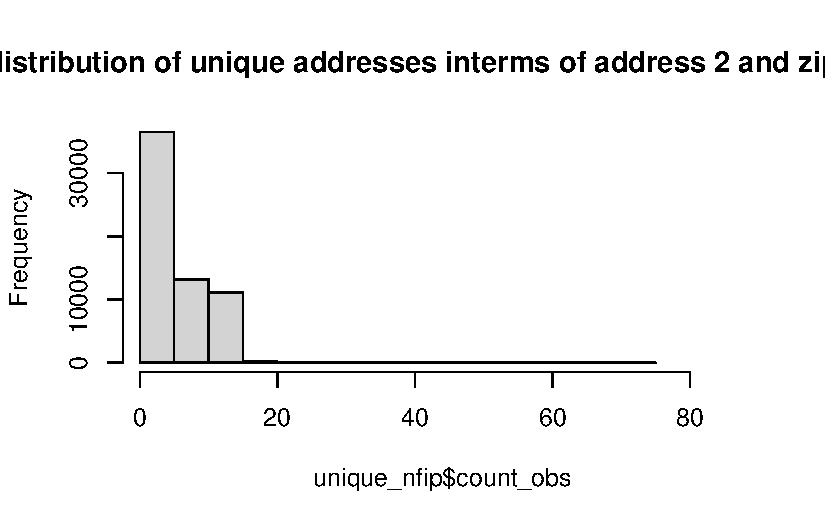
\includegraphics{Gayan_Udugama_Final_Project_files/figure-pdf/unnamed-chunk-7-1.pdf}

}

\end{figure}

\begin{Shaded}
\begin{Highlighting}[]
\FunctionTok{length}\NormalTok{(}\FunctionTok{which}\NormalTok{(unique\_nfip}\SpecialCharTok{$}\NormalTok{count\_obs}\SpecialCharTok{\textgreater{}}\DecValTok{20}\NormalTok{)) }\DocumentationTok{\#\# counting the number of addresses with more than 20 records }
\end{Highlighting}
\end{Shaded}

\begin{verbatim}
[1] 41
\end{verbatim}

\begin{Shaded}
\begin{Highlighting}[]
\CommentTok{\# he plot shows the average insurance premium over time, with a red line demarcating the time when Hurricane Sandy occurred}
\DocumentationTok{\#\# ploting the avarage insurance premium overtime }
\NormalTok{FEAP }\SpecialCharTok{\%\textgreater{}\%}
  \FunctionTok{group\_by}\NormalTok{(year) }\SpecialCharTok{\%\textgreater{}\%} 
  \FunctionTok{summarise}\NormalTok{(}\AttributeTok{mean\_insu =} \FunctionTok{mean}\NormalTok{(t\_premium)) }\SpecialCharTok{\%\textgreater{}\%} 
  \FunctionTok{ggplot}\NormalTok{(}\FunctionTok{aes}\NormalTok{(}\AttributeTok{x =}\NormalTok{ year, }\AttributeTok{y =}\NormalTok{ mean\_insu))}\SpecialCharTok{+}
  \FunctionTok{geom\_point}\NormalTok{()}\SpecialCharTok{+}
  \FunctionTok{geom\_line}\NormalTok{()}\SpecialCharTok{+}
  \FunctionTok{geom\_vline}\NormalTok{(}\AttributeTok{xintercept =} \DecValTok{2013}\NormalTok{, }\AttributeTok{color =} \StringTok{"red"}\NormalTok{) }\SpecialCharTok{+}
  \FunctionTok{xlab}\NormalTok{(}\StringTok{"Year"}\NormalTok{)}\SpecialCharTok{+}
  \FunctionTok{ylab}\NormalTok{(}\StringTok{"Insurance premium ($)"}\NormalTok{)}\SpecialCharTok{+}
  \FunctionTok{labs}\NormalTok{(}\AttributeTok{title =} \StringTok{"Insurance premium over time"}\NormalTok{) }\SpecialCharTok{+}
  \FunctionTok{scale\_x\_discrete}\NormalTok{(}\AttributeTok{limits =} \FunctionTok{unique}\NormalTok{(FEAP}\SpecialCharTok{$}\NormalTok{year)) }\SpecialCharTok{+}
  \FunctionTok{theme}\NormalTok{(}\AttributeTok{text =} \FunctionTok{element\_text}\NormalTok{(}\AttributeTok{size =} \DecValTok{12}\NormalTok{))}
\end{Highlighting}
\end{Shaded}

\begin{figure}[H]

{\centering 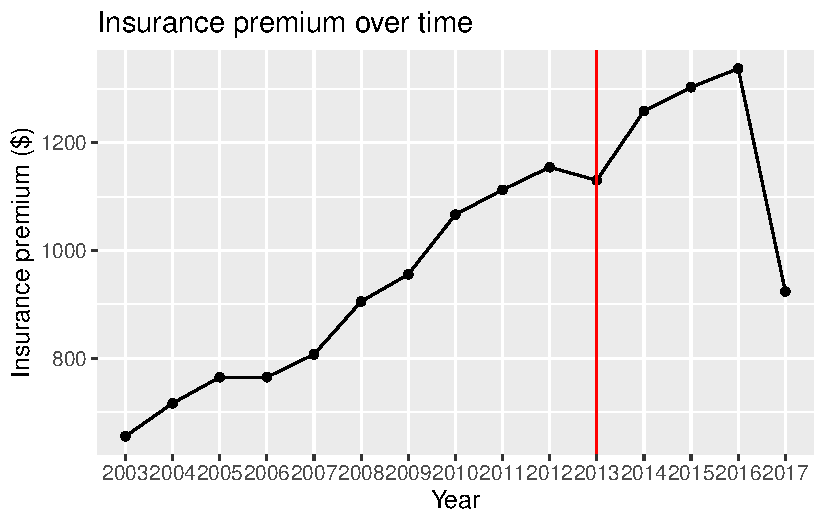
\includegraphics{Gayan_Udugama_Final_Project_files/figure-pdf/unnamed-chunk-9-1.pdf}

}

\end{figure}

\begin{Shaded}
\begin{Highlighting}[]
\DocumentationTok{\#\#\# joining the demographic information into the insurance data at zip code level}

\CommentTok{\# changing variables names to lower case in r}
\FunctionTok{names}\NormalTok{(demo) }\OtherTok{\textless{}{-}} \FunctionTok{tolower}\NormalTok{(}\FunctionTok{names}\NormalTok{(demo))}

\CommentTok{\#renaming the common variable }
\NormalTok{demo }\OtherTok{\textless{}{-}}\NormalTok{ demo }\SpecialCharTok{\%\textgreater{}\%}
  \FunctionTok{rename}\NormalTok{(}\AttributeTok{zip5 =}\NormalTok{ jurisdiction.name)}

\CommentTok{\# join}
\NormalTok{FEAP\_join }\OtherTok{\textless{}{-}} \FunctionTok{left\_join}\NormalTok{(FEAP,demo, }\AttributeTok{by =} \StringTok{"zip5"}\NormalTok{)}
\FunctionTok{head}\NormalTok{(FEAP\_join)}
\end{Highlighting}
\end{Shaded}

\begin{verbatim}
   state_a     county_nm         comm_name    cid address1 address2       city
1 new york  bronx county new york, city of 360497    (b-6)    (b-6)     venice
2 new york  bronx county new york, city of 360497     <NA>    (b-6)         bx
3 new york  bronx county new york, city of 360497     <NA>    (b-6)         bx
4 new york queens county new york, city of 360497     <NA>    (b-6) beechhurst
5 new york queens county new york, city of 360497    (b-6)    (b-6) beechhurst
6 new york queens county new york, city of 360497     <NA>    (b-6) beechhurst
  state_b  zip5 t_premium           occupancy t_cov_bldg t_cov_cont pol_eff_dt
1      fl 34285       369 residential  1  fam     250000     100000 10/24/2016
2      ny 10462      2649 residential  1  fam     213100          0  9/29/2016
3      ny 10465      3326 residential  1  fam     250000      19200 11/30/2016
4      ny 11357      1584   other-residential      87500          0  5/22/2016
5      ny 11357       373 residential  1  fam     250000     100000 10/14/2016
6      ny 11357       415 residential  1  fam     250000     100000  8/20/2016
  pol_exp_dt      gis_geocen   as_of_dt as_of_date pol_eff_date pol_exp_date
1 10/24/2017 1211500240(b-6) 12/31/2016 2016-12-31   2016-10-24   2017-10-24
2  9/29/2017 3600501180(b-6) 12/31/2016 2016-12-31   2016-09-29   2017-09-29
3 11/30/2017 3600501320(b-6) 12/31/2016 2016-12-31   2016-11-30   2017-11-30
4  5/22/2017 3608109870(b-6) 12/31/2016 2016-12-31   2016-05-22   2017-05-22
5 10/14/2017 3608109870(b-6) 12/31/2016 2016-12-31   2016-10-14   2017-10-14
6  8/20/2017 3608109910(b-6) 12/31/2016 2016-12-31   2016-08-20   2017-08-20
  year        occu count.participants count.female percent.female count.male
1 2016 residential                 NA           NA             NA         NA
2 2016 residential                  3            2           0.67          1
3 2016 residential                 21           17           0.81          4
4 2016 residential                  0            0           0.00          0
5 2016 residential                  0            0           0.00          0
6 2016 residential                  0            0           0.00          0
  percent.male count.gender.unknown percent.gender.unknown count.gender.total
1           NA                   NA                     NA                 NA
2         0.33                    0                      0                  3
3         0.19                    0                      0                 21
4         0.00                    0                      0                  0
5         0.00                    0                      0                  0
6         0.00                    0                      0                  0
  percent.gender.total count.pacific.islander percent.pacific.islander
1                   NA                     NA                       NA
2                  100                      0                        0
3                  100                      0                        0
4                    0                      0                        0
5                    0                      0                        0
6                    0                      0                        0
  count.hispanic.latino percent.hispanic.latino count.american.indian
1                    NA                      NA                    NA
2                     1                    0.33                     0
3                    14                    0.67                     0
4                     0                    0.00                     0
5                     0                    0.00                     0
6                     0                    0.00                     0
  percent.american.indian count.asian.non.hispanic percent.asian.non.hispanic
1                      NA                       NA                         NA
2                       0                        0                       0.00
3                       0                        1                       0.05
4                       0                        0                       0.00
5                       0                        0                       0.00
6                       0                        0                       0.00
  count.white.non.hispanic percent.white.non.hispanic count.black.non.hispanic
1                       NA                         NA                       NA
2                        0                       0.00                        2
3                        4                       0.19                        2
4                        0                       0.00                        0
5                        0                       0.00                        0
6                        0                       0.00                        0
  percent.black.non.hispanic count.other.ethnicity percent.other.ethnicity
1                         NA                    NA                      NA
2                       0.67                     0                       0
3                       0.10                     0                       0
4                       0.00                     0                       0
5                       0.00                     0                       0
6                       0.00                     0                       0
  count.ethnicity.unknown percent.ethnicity.unknown count.ethnicity.total
1                      NA                        NA                    NA
2                       0                         0                     3
3                       0                         0                    21
4                       0                         0                     0
5                       0                         0                     0
6                       0                         0                     0
  percent.ethnicity.total count.permanent.resident.alien
1                      NA                             NA
2                     100                              0
3                     100                              1
4                       0                              0
5                       0                              0
6                       0                              0
  percent.permanent.resident.alien count.us.citizen percent.us.citizen
1                               NA               NA                 NA
2                             0.00                2               0.67
3                             0.05               20               0.95
4                             0.00                0               0.00
5                             0.00                0               0.00
6                             0.00                0               0.00
  count.other.citizen.status percent.other.citizen.status
1                         NA                           NA
2                          1                         0.33
3                          0                         0.00
4                          0                         0.00
5                          0                         0.00
6                          0                         0.00
  count.citizen.status.unknown percent.citizen.status.unknown
1                           NA                             NA
2                            0                              0
3                            0                              0
4                            0                              0
5                            0                              0
6                            0                              0
  count.citizen.status.total percent.citizen.status.total
1                         NA                           NA
2                          3                          100
3                         21                          100
4                          0                            0
5                          0                            0
6                          0                            0
  count.receives.public.assistance percent.receives.public.assistance
1                               NA                                 NA
2                                3                               1.00
3                                5                               0.24
4                                0                               0.00
5                                0                               0.00
6                                0                               0.00
  count.nreceives.public.assistance percent.nreceives.public.assistance
1                                NA                                  NA
2                                 0                                0.00
3                                16                                0.76
4                                 0                                0.00
5                                 0                                0.00
6                                 0                                0.00
  count.public.assistance.unknown percent.public.assistance.unknown
1                              NA                                NA
2                               0                                 0
3                               0                                 0
4                               0                                 0
5                               0                                 0
6                               0                                 0
  count.public.assistance.total percent.public.assistance.total
1                            NA                              NA
2                             3                             100
3                            21                             100
4                             0                               0
5                             0                               0
6                             0                               0
\end{verbatim}

\hypertarget{conclusion-and-way-forward}{%
\subsubsection{Conclusion and Way
forward}\label{conclusion-and-way-forward}}

Over time, the insurance premiums have been steadily increasing.
However, there is a slight decrease in premiums in 2013 when Hurricane
Sandy occurred. After 2016, there is a significant reduction in mean
premium value. In the future, I plan to continue this project to
investigate the impact of Hurricane Sandy on insurance premiums, and to
ask more nuanced questions such as how the storm affected minority
communities in New York City.



\end{document}
